\documentclass[5p,authoryear]{elsarticle} 
% other options: preprint, review, 1p, 3p, 5p, 
% bib options: authoryear, number, longtitle,
% other options: times
\usepackage{graphicx}
\usepackage{url}
\usepackage[colorlinks=true,hyperindex=false,bookmarks=false]{hyperref}

\newcommand{\Owlifier}{\textsf{Owlifier}}
\newcommand{\owlifier}{\textsf{owlifier}}

\newcommand{\myblock}[1]{\vspace{12pt}\noindent\textbf{#1}}

\newcommand{\secref}[1]{Section~\ref{#1}}
\newcommand{\figref}[1]{Figure~\ref{#1}}

\title{Owlifier: Creating OWL-DL Ontologies from Simple
  Spreadsheet-Based Knowledge Descriptions\tnoteref{t1}}
\tnotetext[t1]{This work supported in part by NSF grants DBI-0743429
  and DBI-0753144.}

\author[smb]{Shawn Bowers\corref{cor1}}
\ead{sbowers@ucdavis.edu}

\author[jsm]{Joshua S. Madin}
\ead{jmadin@bio.mq.edu.au}

\author[mps]{Mark P. Schildhauer}
\ead[url]{schild@nceas.ucsb.edu}

\cortext[cor1]{Corresponding author}

\address[smb]{Dept. of Computer Science,
 Gonzaga University \& UC Davis Genome Center}

%\address[smb]{UC Davis Genome Center}

\address[jsm]{Dept. of Biological Sciences, Macquarie University, Australia}

\address[mps]{National Center for Ecological Analysis and Synthesis,
  UC Santa Barbara}



\begin{document}

\begin{abstract}
  Discovery and integration of data is important in many ecological
  studies, especially those that concern broad-scale ecological
  questions. Data discovery and integration is often a difficult and
  time-consuming task for researchers, which is due in part to the use
  of informal, ambiguous, and sometimes inconsistent terms for
  describing data content.  Ontologies offer a solution to this
  problem by providing consistent definitions of ecological concepts
  that in turn can be used to annotate, relate, and search for data
  sets.  However, unlike in molecular biology or biomedicine, few
  ontology development efforts exist within ecology. Ontology
  development often requires considerable expertise in ontology
  languages and development tools, which is often a barrier for
  ontology creation in ecology. In this paper we describe an approach
  for ontology creation that allows ecologists to use common
  spreadsheet tools to describe different aspects of an ontology.  We
  present conventions for creating, relating, and constraining
  concepts through spreadsheets, and provide software tools for
  converting these ontologies into equivalent OWL-DL
  representations. We also consider inverse translations, i.e., to
  convert ontologies represented using OWL-DL into our spreadsheet
  format. Our approach allows large lists of terms to be easily
  related and organized into concept hierarchies, and generally
  provides a more intuitive and natural interface for ontology
  development by ecologists.
\end{abstract}

\maketitle


\section{Introduction}

Within the fields of molecular biology and biomedicine considerable
effort has gone into developing ontologies for improving data
discovery and integration
\citep{ashburner00:_gene_ontol,bard04:_ontol_in_biolog}. While similar
benefits can be obtained for ecological data, far fewer efforts exist
to develop broad and consistent terminologies within ecology
\citep{madin08:_advan_ecolog_resear_with_ontol,parr20:_data_sharin_in_ecolog_and_evolut}.
The use of formal ontologies can significantly enhance metadata
descriptions of ecological data. For instance, annotating data with
ontology terms can both help users interpret data as well as enable
advanced capabilities for data discovery and integration, e.g., by
exploiting subsumption and part-of hierarchies as well as more formal
constraints such as cardinality restrictions on properties and term
equivalence \citep{madin08:_advan_ecolog_resear_with_ontol}.

Efforts to engage scientists in the development of ontologies
typically leverage the W3C Web Ontology Language (OWL)
\citep{smith04:_owl_web_ontol_languag_guide} as a standard XML syntax
for representing and sharing ontologies. A key advantage of OWL is
that it is supported by a wide range of generic tools, including
editors
\citep{knublauch04:_editin_descr_logic_ontol_with,kalyanpur05:_swoop},
reasoning systems
\citep{sirin07:_pellet,tsarkov06:_fact_descr_logic_reason}, query
languages
\citep{prudhommeaux08:_sparq_query_languag_for_rdf,motik05:_query_answer_for_owl_dl_with_rules},
and storage technologies
\citep{carroll04:_jena,broekstra02:_sesam}. However, most of these
tools are primarily targeted at experts in knowledge engineering and
software development familiar with the underlying description logic
semantics of OWL-DL \citep{grau08:_owl}. This is especially true with
ontology editors (such as Protege, SWOOP, etc.), which allow for very
detailed ontology specifications, but at the same time require
considerable understanding of the underlying ontology formalisms and
syntax.  The development of the Gene Ontology (GO) has been underway
for over a decade within the molecular biology community, and has lead
to significant improvements in data interoperability by enriching
genomic and biomedical data resources with annotations to
community-based ontologies. A major lesson learned from these efforts
was the importance of keeping the ontology focused, and indeed GO has
a highly delimited scope
\citep{bada04:_short_study_succes_of_gene_ontol}. Ecology, on the
other hand, encompasses an extremely broad range of scales and
disciplines, such that a coordinated ontology development effort would
need to involve a large number of experts to cover the diverse types
of information relevant to ecological investigations.  We believe that
ecological researchers must also begin constructing ontologies for
their own specialized subdisciplines. However, due to the substantial
expertise in formal knowledge representation that is required to use
most existing ontology editing tools, new tools and approaches are
needed to enable the wide-scale creation and adoption of ontologies in
ecology.

This paper presents a novel approach for ontology creation that aims
at being more intuitive for ecologists and that can be used to rapidly
construct large ontologies of ecological terms (classes and
properties). These terms can then be used in subsequent steps to
annotate ecological data (instances), e.g., as in
\citep{bowers08:_concep_model_framew_for_expres,berkley09:_improv_data_discov_metad_repos_seman_searc}.
Our approach is to allow scientists to use common and familiar
spreadsheet-based tools (e.g., Microsoft Excel, Apple Numbers, Open
Office Spreadsheet) to describe, in an intuitive way, different
aspects of an ontology, and then to take these descriptions
(represented as spreadsheets) and convert them into full-fledged OWL
ontologies using a software application called \owlifier.

An \owlifier\ spreadsheet consists of a set of \emph{blocks} that have
a predefined template structure for users to fill in. Each non-empty
row in an \owlifier\ spreadsheet constitutes a block. Each block
defines different aspects of an ontology including classes,
subclasses, synonyms, and properties.  We also provide blocks for
plain-text descriptions of classes and properties, and for referencing
one or more existing ontologies (e.g., to extend an existing ontology
or to define ontology articulations). Blocks can be sparse (inheriting
from previous blocks), which further simplifies the creation of large
ontologies by minimizing the amount of redundant information that must
be provided in the \owlifier\ tabular representation. Several of the
more advanced OWL features are omitted in \owlifier, primarily
associated with properties (e.g., role inclusion axioms, domain and
range property restrictions, and data-type properties among others),
as these can be confusing for non-experts and are more suitable for
experienced knowledge modelers.

While not as expressive as OWL-DL, \owlifier\ can be used to produce
ontology structures that are essential for improved data discovery and
integration \citep{madin07:_ontol_for_descr_and_synth}. Just as
important, because spreadsheet tools are already frequently used by
ecologists to store and analyze data, \owlifier\ can provide
ecologists with a familiar and accessible user interface for ontology
creation. This approach also leverages the easy-to-use interfaces
provided by many spreadsheet tools for organizing and manipulating
tabular data, e.g., via cut/copy/paste, search/replace, sort,
split-window, track-changes, freeze panes, and so on.  In this way, an
ecologist can easily construct (or load) a set of terms, and then
incrementally organize these into class hierarchies, properties, and
constraints.  The use of an editing environment that is familiar to
scientists can significantly help improve the speed and understanding
of ontology construction and avoid the often time-consuming task of
locating, downloading, installing, and learning fundamentally new
software applications and interfaces (e.g., CMAP-COE
\citep{hayes05:_collab_knowl_captur_in_ontol}, Protege
\citep{knublauch04:_editin_descr_logic_ontol_with}). In initial
experiments with ecologists and evolutionary biologists studying trait
data, we found that \owlifier\ enabled them to quickly and easily
comprehend and construct relatively complex and meaningful ontologies.

The rest of this paper is organized as follows. In
\secref{sec:owlifier} we describe the basic syntax and semantics of
\owlifier. The semantics of \owlifier\ blocks is given by mapping
\owlifier\ expressions to description-logic statements. Readers
unfamiliar with description-logic notation may safely ignore these
mappings, focusing instead on the descriptions and examples of blocks
given in \secref{sec:owlifier}.  We define blocks that support a large
subset of OWL-DL and that also generally follow the ontology creation
guidelines defined in \citep{rector04:_owl_pizzas}. We also simplify
certain aspects of ontology creation using OWL, e.g., by assuming
classes are disjoint by default (unless specified otherwise)
\citep{rector04:_owl_pizzas}. In \secref{sec:features} we describe
additional characteristics of \owlifier\ and discuss issues with
respect to classification and reasoning. In
\secref{sec:implementation} we briefly describe the
\owlifier\ implementation, and conclude in \secref{sec:conclusion}
with related and future work. In general, the goal of \owlifier\ is
not to support all constructs in OWL-DL, but instead to provide a
higher-level ontology syntax (via spreadsheet blocks) that is easy for
ecologists to use and understand while also providing the necessary
constructs for developing typical ecological ontologies. By compiling
\owlifier\ to OWL-DL, we also allow for experts to refine and extend
the ontology using more advanced ontology editing tools if necessary
(cf.~\figref{fig:owlifier}).



\section{The Syntax and Semantics of \Owlifier}
\label{sec:owlifier}

As described above, an \owlifier\ table defines an OWL-DL \citep{smith04:_owl_web_ontol_languag_guide} ontology through a set of \emph{blocks} representing one or more ontology definitions.  Each non-empty row in an \owlifier\ table corresponds to a block. The type of the block is given in the first column of the row.
% This section describes in detail each type of block supported by
% \owlifier.
We assume that if any properties or classes used in a block are not imported from another ontology, then they are to be added to the ontology being specified by the \owlifier\ table (i.e., the ``current'' ontology). In general, we name blocks according to the terms used in \citep{bowers08:_concep_model_framew_for_expres,madin07:_ontol_for_descr_and_synth} as opposed to the names used for corresponding constructs in OWL-DL. This choice of block names helps to simplify terminology (e.g., we use ``relationship'' below instead of ``object property''), allows \owlifier\ to easily generate ontologies that extend the observational model of \citep{bowers08:_concep_model_framew_for_expres,madin07:_ontol_for_descr_and_synth}, and avoids confusion with established terms commonly used within ecology (e.g., ``class'').

\myblock{Import Blocks.} Import blocks assign namespace labels to
external ontologies. Each external ontology is imported into the
current ontology. We refer to the ontologies of import blocks as
\emph{imported ontologies}.  Using import blocks, classes and
properties of imported ontologies can be used within other blocks of
an \owlifier\ table.  Rows containing import blocks take the form
\begin{itemize}
\item[]
  \begin{tabular}{|l|l|l|}\hline
    \textsf{import} & $n$ & $u$ \\ \hline 
  \end{tabular} 
\end{itemize}
where $n$ is a namespace label and $u$ is an OWL ontology URI. Classes
and properties from imported ontologies are referenced by prefixing
the namespace label $n$ to the corresponding class or property name in
the normal way. As an example, the following block imports the SWEET
``Earth Realm'' ontology \citep{raskin05}.
\begin{small}
\begin{tabbing}
  ~~\textsf{import}  \textsf{sweet} 
  \textsf{http://sweet.jpl.nasa.gov/ontology/earthrealm.owl}
\end{tabbing}
\end{small}
With this import block the class denoting Marine Ecosystems (a class
defined in the SWEET ontology) can be referred to from within an
\owlifier\ table using the expression
\textsf{sweet:MarineEcosystem}. Because this class refers to a class
in another ontology, we refer to it as an \emph{imported class}.


\myblock{Entity Blocks.} Entity blocks are the primary blocks used to
define ontologies. An entity block introduces new OWL classes and
specifies subclass relationships. Imported classes may also be used
within entity blocks by prefixing class names with namespace labels
(as described above).  Rows containing entity blocks take the form
\begin{itemize}
\item[] 
  \begin{tabular}{|l|l|l|l|l|}\hline
   \textsf{entity} & $c_1$ & $c_2$ & \dots & $c_n$ \\ \hline 
  \end{tabular} \hfill ($n \ge 1$)
\end{itemize}
where each class $c_i$ is asserted in the current ontology to subsume
$c_{i+1}$, for $1 \le i < n$. That is, each $c_i$ in an entity block
induces the description logic axiom $c_{i+1} \sqsubseteq c_i$.  If
both $c_i$ and $c_{i+1}$ are imported classes, we say that the block
defines an ``articulation'' (i.e., mapping) between the two
classes. The following entity block defines a simple subclass
hierarchy.
\begin{tabbing}
  ~~\textsf{entity} \textsf{PhysicalFeature} 
    \textsf{AquaticPhysicalFeature} \textsf{River}
\end{tabbing}
This block states that Physical Feature, Aquatic Physical Feature, and
River are classes; River is a subclass of Aquatic Physical Feature;
and Aquatic Physical Feature is a subclass of Physical Feature. The
following entity block introduces a new class via an imported class.
\begin{tabbing}
  ~~\textsf{entity} \textsf{sweet:MarineEcosystem} 
    \textsf{IntertidalEcosystem}
\end{tabbing}
This block states that Intertidal Ecosystem is a subclass of the
Marine Ecosystem class imported from the SWEET ontology. Similarly,
assuming ``marine'' denotes an existing ontology of marine ecosystem
concepts, the following block defines a simple class articulation.
\begin{tabbing}
  ~~\textsf{entity} \textsf{sweet:MarineEcosystem} 
    \textsf{marine:DeepSeaEcosystem}
\end{tabbing}
This block states that the Deep Sea Ecosystem class of the marine
ontology is a subclass of the Marine Ecosystem class of the SWEET
ontology (thus defining a mapping between these two ontologies).


\myblock{Synonym Blocks.} Synonym blocks define equivalence
relationships between ontology classes.  Rows containing synonym
blocks take the form
\begin{itemize}
\item[] 
  \begin{tabular}{|l|l|l|l|l|}\hline
    \textsf{synonym} & $c_1$ & $c_2$ & \dots & $c_n$ \\ \hline 
  \end{tabular} \hfill ($n \ge 2$)
\end{itemize}
where each class $c_i$ is equivalent to class $c_{i+1}$ in the current
ontology, for $1 \le i < n$. That is, each $c_i$ in a synonym block
induces a description logic axiom of the form $c_i \equiv
c_{i+1}$. The following synonym block creates a simple equivalence
relationship.
\begin{tabbing}
  ~~\textsf{synonym} \textsf{Maize} \textsf{Corn}
\end{tabbing}
This block states that the Maize and Corn classes are synonyms
(equivalent classes). Similar to entity blocks, synonym blocks often
contain imported classes for extending existing ontologies or defining
ontology mappings.


\myblock{Overlap Blocks.} Except in certain situations (described
further in \secref{sec:features}), classes are generally
assumed to be disjoint in \owlifier.  Overlap blocks explicitly relax this assumption by
stating that a given set of classes may share common instances. Rows containing overlap blocks take the form
\begin{itemize}
\item[]
  \begin{tabular}{|l|l|l|l|l|}\hline
    \textsf{overlap} & $c_1$ & $c_2$ & \dots & $c_n$ \\ \hline 
  \end{tabular} \hfill ($n \ge 2$)
\end{itemize}
where each class $c_i$ is allowed to share instances with each class
$c_j$, for $1 \le i,j \le n$. That is, a given $c_i$ and $c_j$ in an
overlap block are not defined to be disjoint classes in the current
ontology. As an example, consider the following entity blocks that
define the classes Estuary, Lagoon, and Marsh as subclasses of
Ecological Habitats.
\begin{tabbing}
  ~~\textsf{entity} \textsf{EcologicalHabitat} \textsf{Estuary} \\ 
  ~~\textsf{entity} \textsf{EcologicalHabitat} \textsf{Lagoon} \\ 
  ~~\textsf{entity} \textsf{EcologicalHabitat} \textsf{Marsh} 
\end{tabbing}
Given only these blocks, \owlifier\ treats Estuary, Lagoon, and Marsh
as disjoint classes. To relax this assumption and allow, e.g., types
of Lagoons to also be types of Estuaries, we explicitly add the
following overlap block
\begin{tabbing}
  ~~\textsf{overlap} \textsf{Estuary} \textsf{Lagoon}
\end{tabbing}
In general, overlap blocks are rarely used but provide a mechanism to
override the default behavior of \owlifier\ in asserting disjoint
classes.

% \myblock{Property Blocks.} Property blocks define basic object property
% domain and range constraints. , where the domain of an
% object property denotes the set of individuals that can have the
% property, and the range denotes the set of individuals that can be
% related to domain individuals through the property. Rows containing
% relationship blocks take the form 
% \begin{itemize}
% \item[]
%   \begin{tabular}{|l|l|l|l|}\hline \textsf{property} & $p$ & $c_1$
%     & $c_2$ \\ \hline
%   \end{tabular} \hfill ($n \ge 2$)
% \end{itemize}
% where $p$ is the object property, class $c_1$ is the property domain,
% and class $c_2$ is the property range. 

\myblock{Relationship Blocks.} Relationship blocks define
\emph{required} class object properties.  An object property within
OWL is a property defined between two class instances. Rows containing
relationship blocks take the form
\begin{itemize}
\item[]
  \begin{tabular}{|l|l|l|l|l|l|}\hline \textsf{relationship} & $p$ & $c_1$
    & $c_2$ & \dots & $c_n$ \\ \hline
  \end{tabular} \hfill ($n \ge 2$)
\end{itemize}
where $p$ is an object property and each $c$ is a class.  For every
class $c_i$, the relationship block induces the description logic axiom $c_i
\sqsubseteq \exists p . c_{i+1}$ stating that each instance of $c_i$
is $p$-related to some instance of $c_{i+1}$, for $1 \le i < n$.  For
example, the following block states that instances of the class
California Voles live in Grassy Areas.
\begin{tabbing}
  ~~\textsf{relationship} \textsf{livesIn} \textsf{CaliforniaVole} 
    \textsf{GrassyArea}
\end{tabbing}
In some cases, a particular property can apply to a sequence of
classes, and for convenience, each such class can be specified in
\owlifier\ using a single block. For example, consider the following
block.
\begin{small}
\begin{tabbing}
  ~~\textsf{relationship} \textsf{directlyBelow} \textsf{Hypolimnion} 
    \textsf{Thermocline} \textsf{Epilimnion} 
\end{tabbing}
\end{small}
This block states that, e.g., within a thermally stratified lake, the
Hypolimnion layer is directly below the Thermocline layer, and the
Thermocline layer is directly below the Epilimnion layer. 

\myblock{Transitive Blocks.} Transitive blocks are special cases of
relationship blocks where the object property is asserted to be
transitive. That is, if a property $p$ is declared to be transitive,
and $p$ relates an individual $x$ to an individual $y$ and $y$ to an
individual $z$, then $p$ is assumed to also relate $x$ to $z$. Rows
containing transitive blocks take the form
\begin{itemize}
\item[]
  \begin{tabular}{|l|l|l|l|l|l|}\hline \textsf{transitive} & $p$ & $c_1$
    & $c_2$ & \dots & $c_n$ \\ \hline
  \end{tabular} \hfill ($n \ge 2$)
\end{itemize}
where $p$ is an object property and each $c$ is a class.  The
following block is a simple example of a transitive relationship
definition.
\begin{tabbing}
  ~~\textsf{transitive} \textsf{hasPart} \textsf{Body}
  \textsf{Head} \textsf{Eye} \textsf{Retina}
\end{tabbing} 
This block states that every instance of the class Body has a Head as
a part, every instance of the class Head has an Eye as a part, and
every instance of the class Eye has a Retina as a part. Moreover,
because the \textsf{hasPart} property above is defined to be
transitive, it is possible to infer that every instance of Body also
has an Eye and a Retina as a part through the inherited relationship
restrictions $\textsf{Body} \sqsubseteq \exists \textsf{hasPart}
. \textsf{Head}$, $\textsf{Head} \sqsubseteq \exists \textsf{hasPart}
. \textsf{Eye}$, and $\textsf{Eye} \sqsubseteq \exists
\textsf{hasPart} . \textsf{Retina}$.


\myblock{Cardinality Blocks.} Cardinality blocks are also similar to
relationship blocks.  We consider three types of cardinality blocks
for defining minimum, maximum, and exact cardinality restrictions.
Rows containing minimum blocks take the form
\begin{itemize}
\item[]
  \begin{tabular}{|l|l|l|l|l|l|l|}\hline \textsf{min} & $p$ & $m$ & 
    $c_1$ & $c_2$ & $\dots$ & $c_n$
    \\ \hline 
  \end{tabular} \hfill $(n \ge 2)$
\end{itemize}
where $m$ is the minimum number of properties $p$ that instances of
class $c_i$ must have to instances of concept $c_{i+1}$, for $1 \le i
< n$.  For each class $c_i$, a minimum cardinality block induces the
description logic axiom $c_{i} \sqsubseteq \; (\le m) \; p.c_{i+1}$
stating that each instance of $c_i$ must be $p$-related to at least
$m$ unique instances of $c_{i+1}$. The following two blocks
demonstrate simple minimum cardinality constraints.
\begin{tabbing}
  ~~\textsf{min} \textsf{hasPart} 1 \textsf{Body} \textsf{Head} 
  \textsf{Nose} \\
  ~~\textsf{min} \textsf{hasPart} 2 \textsf{Head} \textsf{Eye}
\end{tabbing}
The first block states that instances of the class Body have at least
one Head as a part, which in turn have at least one Nose as a
part.\footnote{Cardinality restrictions ensuring participation to at
  least one property are typically not given through minimum
  cardinality blocks since they are also implied by relationship
  blocks.} The second block states that instances of the class Head
have at least two Eyes as parts. 

Rows containing maximum blocks take the form
\begin{itemize}
\item[]
  \begin{tabular}{|l|l|l|l|l|l|l|}\hline \textsf{max} & $p$ & $m$ & 
    $c_1$ & $c_2$ & $\dots$ & $c_n$
    \\ \hline
  \end{tabular} \hfill $(n \ge 2)$
\end{itemize}
where $m$ is the maximum number of properties $p$ that instances of
concept $c_i$ may have to instances of concept $c_{i+1}$, for $1 \le i
< n$.  For each class $c_i$, a maximum cardinality block induces the
description logic axiom $c_i \sqsubseteq \; (\ge m) \; p.c_{i+1}$
stating that each instance of $c_i$ may be $p$-related to at most $m$
unique instances of $c_{i+1}$. The following two blocks demonstrate
simple maximum cardinality constraints.
\begin{tabbing}
  ~~\textsf{max} \textsf{hasPart} 1 \textsf{Body} \textsf{Head} 
  \textsf{Nose} \\
  ~~\textsf{max} \textsf{hasPart} 2 \textsf{Head} \textsf{Eye}
\end{tabbing}
The first block states that instances of the class Body have at most
one Head as a part, which in turn has at most one Nose as a part. The
second block states that instances of the class Head have at most two
Eyes as parts. 

Rows containing exact blocks take the form
\begin{itemize}
\item[]
  \begin{tabular}{|l|l|l|l|l|l|l|}\hline \textsf{exact} & $p$ & $m$ & 
    $c_1$ & $c_2$ & $\dots$ & $c_n$
    \\ \hline
  \end{tabular} \hfill $(n \ge 2)$
\end{itemize}
where $m$ is the number of properties $p$ that instances of concept
$c_i$ must have to instances of concept $c_{i+1}$, for $1 \le i < n$.
For each class $c_i$, an exact block induces the description logic
axiom $c_i \sqsubseteq \; (= m) \; p.c_{i+1}$ stating that each
instance of $c_i$ must be $p$-related to $m$ unique instances of
$c_{i+1}$.

\myblock{Inverse Blocks.} Inverse blocks state that two object
properties are inverses of each other. If $p_1$ and $p_2$ are defined
to be inverse properties, whenever $p_1$ relates an individual $x$
to an individual $y$ then $p_2$ (as the inverse of $p_1$) is assumed
to relate $y$ to $x$.  Rows containing inverse blocks take the
form
\begin{itemize}
\item[]
  \begin{tabular}{|l|l|l|}\hline \textsf{inverse} & $p_1$ & $p_2$
\\ \hline
  \end{tabular}
\end{itemize}
where $p_1$ and $p_2$ are object properties. A common example of
inverse properties are \textsf{hasPart} and \textsf{partOf}, i.e., if
an individual $x$ has an individual $y$ as a part, then $y$ is
by definition a part of $x$.


% \myblock{Attribute Blocks.} Attribute blocks define required
% \emph{datatype} properties of classes. Unlike object properties, a
% datatype property within OWL is a property defined between a class
% instance and a literal value (e.g., a string or integer). Rows
% containing attribute blocks take the form
% \begin{itemize}
% \item[]
%   \begin{tabular}{|l|l|l|l|l|l|l|}\hline \textsf{attribute} & $p$ & $c_1$
%     & $c_2$ & \dots & $c_n$ \\ \hline
%   \end{tabular} \hfill ($n \ge 1$)
% \end{itemize}
% where $p$ is a datatype property and $c_i$ is a class, for $1 \le i
% \le n$. For each concept $c_i$, the attribute block induces the
% description logic axiom $c_i \sqsubseteq \exists p$ stating that
% each instance of $c_i$ has, amongst possibly other things, a
% property $p$ with a literal value. Attributes are often useful for
% As an example, the following ...


% \myblock{Value Blocks.} Value blocks define required datatype property
% \emph{constant values} for concepts. A value block has the form
% \begin{itemize}
% \item[]
%   \begin{tabular}{|l|l|l|l|l|l|l|}\hline \textsf{value} & $P$ & $V$ & $C_1$
%     & $C_2$ & \dots & $C_n$ \\ \hline
%   \end{tabular} \hfill ($n \ge 1$)
% \end{itemize}
% where $P$ is a datatype property, $C_i$ is a concept for $1 \le i \le
% n$, and $V$ is a datatype value. For each concept $C_i$, the value
% block induces the DL axiom \[C_i \sqsubseteq (V \in P)\] stating that
% each instance of $C_i$ has a value $V$ for property $P$.  The value
% restrictions stated by value blocks are often used for defining
% so-called \emph{value partitions} \citep{co-ode}.


\myblock{Sufficient Blocks.} Sufficient blocks are similar to synonym
blocks in that they state equivalences between classes. We consider
two types of sufficient blocks. A sufficient entity block takes the
form
\begin{itemize}
\item[]
  \begin{tabular}{|l|l|l|l|l|l|}\hline \textsf{sufficient} & \textsf{entity} & $c_1$ & $c_2$ & \dots & $c_n$
\\ \hline
\end{tabular} \hfill ($n \ge 2$)
\end{itemize}
where each $c_i$ is a class. A sufficient entity block induces the
description logic axiom $c_1 \equiv c_2 \sqcap \dots \sqcap c_n$
stating that the class $c_1$ is equivalent to the intersection of the
classes $c_2$ through $c_n$.  Similarly, a sufficient relationship
block takes the form
\begin{itemize}
\item[]
  \begin{tabular}{|l|l|l|l|l|l|l|l|}\hline \textsf{sufficient} & \textsf{relationship} & (\textsf{not}) & $p$ & $c_1$ & $c_2$ \\ 
\hline \end{tabular} 
\end{itemize} 
where $p$ is an object property, $c_1$ and $c_2$ are classes, and
\textsf{not} is an optional qualifier.  A sufficient relationship
block (without a \textsf{not} qualifier) induces the description logic
axiom $c_1 \equiv \exists p . c_2$ stating that the class $c_1$ is
equivalent to the set of individuals that are $p$-related to at least
one individual of class $c_2$. The \textsf{not} qualifier states that
the absence of the property is a defining characteristic of the
class. Thus, a sufficient relationship block containing a \textsf{not}
qualifier induces the description logic axiom $c_1 \equiv \neg \exists
p . c_2$.  The use of multiple sufficient blocks for a particular
class results in a single axiom in which each constraint (i.e., class
constructor) is combined via intersection ($\sqcap$). For example, the
following blocks
\begin{small}
\begin{tabbing}
~~\textsf{sufficient} \= \textsf{relationship} \= \textsf{Eutheria} \=
  \textsf{Mammal} \= \kill ~~\textsf{sufficient} \>
  \textsf{relationship} \> \textsf{hasPart} \> \textsf{Mammal} \>
  \textsf{Hair} \\ ~~\textsf{sufficient} \> \textsf{entity} \>
  \textsf{Eutheria} \> \textsf{Mammal} \\ ~~\textsf{sufficient} \>
  \textsf{relationship} \> \textsf{not} \> \textsf{hasPart} \>
  \textsf{Eutheria} \textsf{EpipubicBone}
\end{tabbing}
induce the following description logic axioms.
\begin{tabbing}
~~$\textsf{Mammal} \equiv \exists \textsf{hasPart}.\textsf{Hair}$\\ 
~~$\textsf{Eutheria} \equiv \textsf{Mamma} \sqcap \neg \exists \textsf{hasPart} . \textsf{EpipubicBone}$
\end{tabbing}
\end{small}
These axioms state that \emph{any} individual that has Hair as a part
is a Mammal and that \emph{any} Mammal that does not have an Epipubic
Bone as a part is a Eutheria.

\myblock{Comment Blocks.} There are two types of comment blocks that
each provide a mechanism to add plain-text comments to
\owlifier\ tables. A description block attaches a plain-text comment
to classes and properties. Rows containing description blocks take the
form
\begin{itemize}
\item[]
  \begin{tabular}{|l|l|l|}\hline \textsf{description} & $c$ or $p$ & $s$
    \\ \hline
  \end{tabular}
\end{itemize}
where the string $s$ is associated as a comment to the class $c$ or
property $p$. A note block attaches comments to the current
ontology. Rows containing note blocks can occur anywhere within an
\owlifier\ table, and take the form
\begin{itemize}
\item[]
  \begin{tabular}{|l|l|l|}\hline \textsf{note} & $s$
\\ \hline
  \end{tabular}
\end{itemize}
where $s$ is a comment string. 


\section{Additional Features of \Owlifier}
\label{sec:features}

Here we briefly describe some of the additional features of \owlifier,
specifically focusing on the use of disjoint classes,
\owlifier\ reasoning, and additional block syntax.
 
\subsection{Disjoint Class Inference}

OWL is based on the open world assumption, which can lead to a number
of ontology development ``pitfalls'' for those new to the language
\citep{smith04:_owl_web_ontol_languag_guide,rector04:_owl_pizzas}. One
example is in the creation of disjoint classes.  In particular, unless
explicitly asserted, distinct classes within an OWL-DL ontology are
not assumed to be disjoint. However, in many ontologies a large number
of classes are typically defined as being disjoint (e.g., sibling
classes), and stating these disjoint constraints is often time
consuming since each pair of classes must be given an explicit
disjoint assertion. Editors such as Protege
\citep{knublauch04:_editin_descr_logic_ontol_with} provide shortcuts
via the user interface to create specific sets of disjoint assertions,
e.g., by allowing a user to define all children of a particular class
as disjoint. In general, however, many users expect such classes to be
disjoint by default \citep{rector04:_owl_pizzas} and this expectation
often leads to modeling errors.

Alternatively, the default assumption in \owlifier\ is that distinct
classes are disjoint. Specifically, as an \owlifier\ table is
converted to an OWL-DL ontology, the system analyzes the class
hierarchy structure and identifies pairs of classes that are: (1) not
related via subclass relations (either direct or indirect subclasses);
(2) not defined as synonyms; and (3) not explicitly defined to overlap
via an overlap block. Each such pair of classes is then asserted by
\owlifier\ in the resulting ontology as being disjoint. As described
in \citep{rector04:_owl_pizzas}, undeclared disjoint classes are a
common problem in ontology development using OWL-DL and often limit
the utility of reasoning systems (by limiting the inferences that can
be obtained). The approach employed in \owlifier\ for handling
disjoint classes makes the common expectations of users the default
case, which in general should lead to a more intuitive ontology
editing environment and an overall fewer number of modeling mistakes.



\begin{figure*}
  \centering
  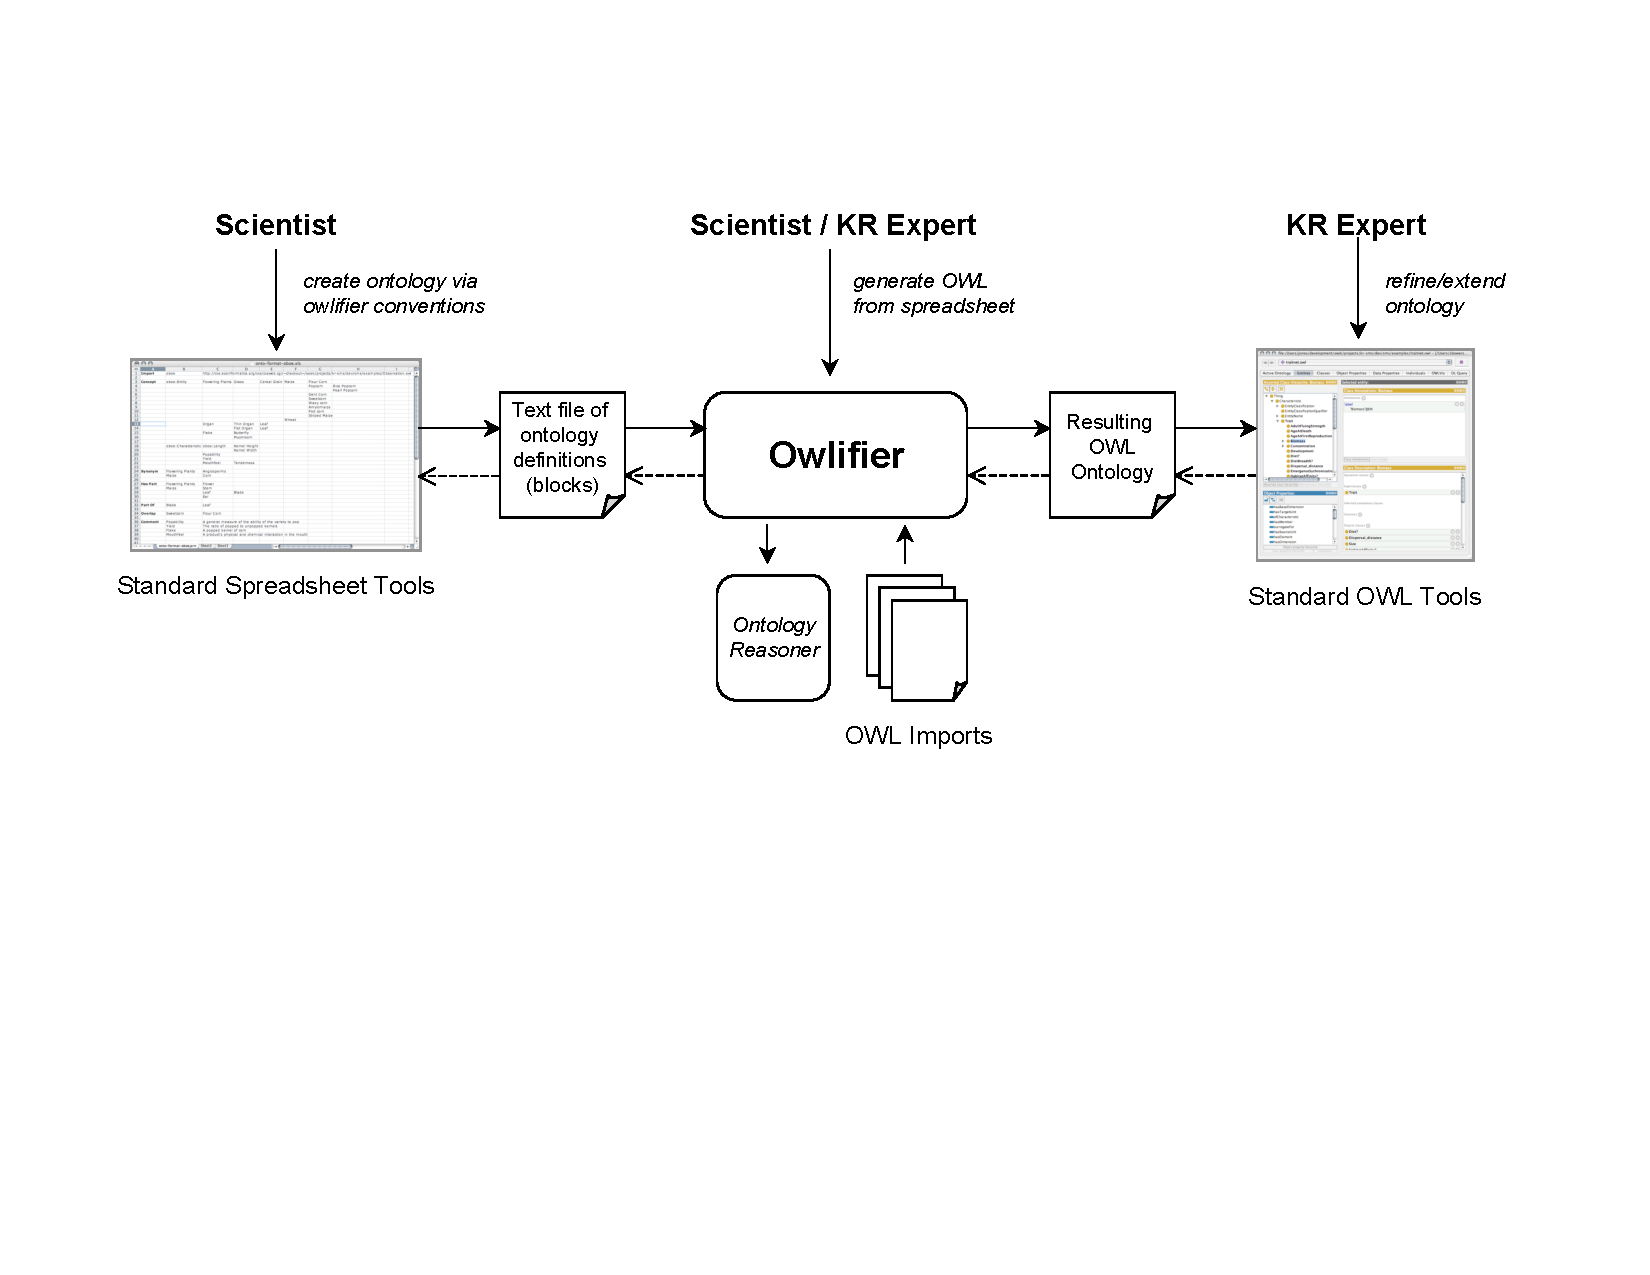
\includegraphics[scale=.75]{architecture.pdf}
  \caption{The basic \owlifier\ application and relation to other
    technologies.}
  \label{fig:owlifier}
\end{figure*}



\subsection{Reasoning in \Owlifier}

Blocks in \owlifier\ are unambiguous, i.e., for every \owlifier\ block
(or set of blocks in the case of sufficient blocks) there is a
well-defined set of corresponding OWL-DL axioms. This property is
important because it implies that reasoning can be performed over
ontologies defined in \owlifier\ using standard OWL-DL reasoners.  We
use this capability in our current \owlifier\ implementation
(described further in \secref{sec:implementation}) to verify
ontologies defined using \owlifier\ and report possible errors to
users.

In general, new axioms are inferred from an \owlifier\ ontology
primarily from the use of synonym blocks, sufficient blocks, and
transitive blocks (whose inferences are described in the previous
section). For instance, let $A$, $B$, and $C$ be classes and $P$ be an
object property. From an axiom $A \equiv B$ generated from a synonym
block, and an axiom $B \sqsubseteq \exists P.C$ generated from a
relationship block, the axiom $A \sqsubseteq \exists P.B$ would be
inferred. Thus, the axioms of a particular class are ``inherited'' by
all of the synonyms of the class. Similarly, from an axiom $A \equiv
\exists P. C$ generated from a sufficient block, and an axiom $B
\sqsubseteq \exists P.C$ generated from a relationship block, the
axiom $B \sqsubseteq A$ would be inferred. For both the case of
synonym and sufficient blocks, the use of equivalence permits a number
of additional inferences to be made via an OWL-DL reasoner.

As described in \citep{rector04:_owl_pizzas} additional reasoning can
occur within OWL-DL ontologies when domain and range axioms are
provided (as well as, e.g., property closure axioms).  We explicitly
do not consider these constraints in the current version of
\owlifier\ because they also often result in modeling errors for
inexperienced OWL-DL users \citep{rector04:_owl_pizzas}. Instead, we
adopt the approach of more traditional description logics, which do
not have explicit domain and range axioms.  Although not currently
supported in \owlifier, domain and range constraints as well as
property closure axioms can be inferred from given relationship
blocks.

\subsection{Sparse Blocks} 

To help simplify the creation of class hierarchies and property
sequences (including transitive, cardinality, and sufficient blocks),
we allow for ``sparse'' blocks that inherit missing information from
their closest proceeding block. For instance the following entity
blocks
\begin{tabbing}
  ~~\textsf{entity} \= \textsf{EcologicalHabitat} \= \textsf{Estuary} \= \kill
  ~~\textsf{entity} \> \textsf{EcologicalHabitat} \> \textsf{Estuary} \> 
  \textsf{Bay}\\
  ~~\textsf{entity} \> \textsf{EcologicalHabitat} \> \textsf{Estuary} \>
  \textsf{Fjord} \\
  ~~\textsf{entity} \> \textsf{EcologicalHabitat} \> \textsf{Marsh} \>
  \textsf{TidalMarsh} \\ 
  ~~\textsf{entity} \> \textsf{EcologicalHabitat} \> \textsf{Marsh} \>
  \textsf{SaltMarsh}
\end{tabbing}
can be equivalently represented in \owlifier\ using the following
sparse blocks.
\begin{tabbing}
  ~~\textsf{entity} \= \textsf{EcologicalHabitat} \= \textsf{Estuary} \= \kill
  ~~\textsf{entity} \> \textsf{EcologicalHabitat} \> \textsf{Estuary} \> 
  \textsf{Bay}\\
  \> \> \> \textsf{Fjord} \\
  \> \> \textsf{Marsh} \> \textsf{TidalMarsh} \\ 
  \> \> \> \textsf{SaltMarsh}
\end{tabbing}
In general, the use of sparse blocks simplifies ontology creation by
not requiring users to enter every redundant field explicitly, which
in turn can simplify the overall layout of the ontology within a
spreadsheet.  Additionally, \owlifier\ does not place constraints on
the order of blocks within a spreadsheet. Classes also do not need to
be explicitly defined within an entity block, e.g., classes without
corresponding entity blocks can be introduced simply through synonym
and relationship blocks. This typically occurs when a particular class
does not participate as a subclass or superclass of another class in
the current ontology. Taken together, these approaches allow users to
enter minimal information by limiting redundancy and by supporting a
range of inferences, while at the same time reducing the causes of
many errors commonly made in ontology development by non-experts.



\section{The \Owlifier\ Implementation}
\label{sec:implementation}

\figref{fig:owlifier} shows the general architecture of the
\owlifier\ application. A scientist first creates a spreadsheet
containing a set of ontology definitions using \owlifier\ conventions.
The spreadsheet is then exported as a plain-text file containing the
\owlifier\ table, e.g., using a CSV or tab-delimited format. The
\owlifier\ table is then sent to the \owlifier\ application, which
performs a number of steps that include: (i) parsing the file; (ii)
generating the corresponding OWL-DL representation (e.g., in the
current implementation, the OWL-API is used
\citep{horridge07:_ignit_owl}, although Jena \citep{carroll04:_jena}
could be used as well); (iii) validating the ontology and ensuring it
is consistent via an OWL-DL reasoner (e.g., the current implementation
uses Pellet \citep{sirin07:_pellet}); and (iv) outputting the
corresponding OWL-DL file. The resulting OWL file can then be refined
and extended via existing OWL tools (e.g., Protege or SWOOP). It is
also possible for the refined ontology to be converted back to a
corresponding \owlifier\ representation (shown using dashed lines in
\figref{fig:owlifier}). While straightforward to perform, this
``back'' conversion is not information preserving since not all OWL-DL
statements can be represented through \owlifier\ blocks.  That is, the
conversion from OWL-DL to \owlifier\ will only preserve OWL-DL
constructs that are represented by \owlifier\ blocks.  In particular,
\owlifier\ does not support a number of OWL-DL language constructs,
including domain and range constraints, datatype properties, sub
properties, property constraints (i.e., functional, symmetric, and
inverse functional), value restrictions, individuals, etc., as well as
various combinations of OWL-DL constructs.

The current implementation of \owlifier\ is written as an open-source
Java application\footnote{See
  \url{https://semtools.ecoinformatics.org/owlifier}} and supports a
subset of the blocks defined in \secref{sec:owlifier}. In particular,
we are currently extending \owlifier\ to fully support sufficient
blocks (the remaining blocks described in \secref{sec:owlifier} are
implemented) as well as the potentially lossy, back conversion from
OWL-DL files to corresponding \owlifier\ blocks. The current
implementation of \owlifier\ is being used within a project focused on
integrating vegetation trait data.  As noted above, not all the blocks
described here are yet supported, however, these priority needs are
clearly emerging from our interactions with the vegetation scientists.
Nevertheless, these scientists were able to rapidly prototype and
revise their trait ontologies using \owlifier, with little to no
instruction in formal logic or knowledge modeling.  In addition,
\owlifier\ is being used to construct term hierarchies from large sets
of keywords (harvested from existing metadata documents) as well as to
define articulations between existing ontologies and the observation
ontology defined in \citep{madin07:_ontol_for_descr_and_synth}. As we
continue to use \owlifier\ within these projects, we intend to extend
the application as needed to support additional blocks and services.


\section{Conclusion}
\label{sec:conclusion}

This paper presents a new approach for developing ontologies to
address barriers in ontology development and adoption by
ecologists. Our approach allows scientists to use familiar spreadsheet
software (e.g., frequently used by ecologists for storing and
analyzing data) to create ontologies by filling in a set of templates,
or blocks, that generate OWL-DL class hierarchies, properties, and
constraints via the \owlifier\ application.  This approach can provide
a more intuitive and accessible ontology editing environment for
ecologists, especially compared to existing OWL-based tools that
require considerable expertise in the underlying logic
formalisms. Similar to standard OWL ontologies,
\owlifier\ spreadsheets can import and extend existing OWL-DL
ontologies (including those generated from \owlifier\ spreadsheets),
which further supports the community development and interoperability
of ontologies. Blocks in \owlifier\ (or similarly, partially filled in
blocks) can also be reused during ontology creation to help ensure
that future ontology development adheres to best practices and
community standards (e.g., similar to ``part-of'' properties defined
in the Gene Ontology
\citep{bada04:_short_study_succes_of_gene_ontol}).

Protege provides a variety of ontology editing plug-ins, including a
simple interface for text-based editing of class hierarchies. In
\citep{kola07:_impor_spread_data_into_proteg}, an approach is
described for importing spreadsheet-based ontology descriptions into
Protege. However, this approach aims at supporting \emph{ad-hoc}
spreadsheet structures by providing an intermediate interface for
mapping these structures into ontology axioms. This approach is
similar to others (e.g.,
\citep{han08:_rdf12,bizer03:_d2r_map,an06:_discov_seman_of_relat_tables_throug_mappin})
for defining mappings from relational data to RDF and OWL ontology
class and instance data. In addition to these approaches, a number of
visual editing environments have been developed to help novice users
create OWL-based ontologies (e.g.,
\citep{hayes05:_collab_knowl_captur_in_ontol}). To the best of our
knowledge, however, our approach is the first to consider an intuitive
spreadsheet-based approach together with a detailed set of templates
that can support a large subset of existing OWL constructs. In
addition, we define a number of shortcuts for creating
\owlifier\ tables, including sparse blocks and default semantics
(e.g., disjoint classes) that further simplify ontology creation for
end users.

As future work, we plan to extend our current
\owlifier\ implementation to support the full set of blocks defined
here as well as introduce additional blocks, e.g., for creating OWL
datatype properties. We also would like to explore approaches for
supporting round-trip conversions between \owlifier\ tables and OWL-DL
ontologies that allow scientists and knowledge-representation experts
to incrementally develop \owlifier-based ontologies.  Specifically, we
want to extend the \owlifier\ application so that it can store and
re-apply changes made by knowledge-representation experts that
previously modified an OWL-DL ontology generated by \owlifier. For
instance, if an OWL-DL ontology generated from an
\owlifier\ spreadsheet is refined and extended by a
knowledge-representation expert, then converted back into an
\owlifier\ ontology that is further edited and extended by a
scientist, and then converted again into an OWL-DL ontology, we want
to maintain (i.e., re-apply) the original extensions and edits created
by the knowledge-representation expert that are still relevant (thus
supporting lossless conversions).  We also plan to extend the
\owlifier\ application to support translation into the observation
ontology framework presented in
\citep{bowers08:_concep_model_framew_for_expres} and perform
additional testing and evaluation of the \owlifier\ approach with a
wide range of ecologists.

%\bibliographystyle{elsarticle-num}
\bibliographystyle{abbrvnat} 
\bibliography{main}


\end{document}

